\chapter{Results}
%comparaison, metriques. graphs

\section{Time Series Approach}
As the methodology to arrive to the final model is the same in R and Python, we will just layout the Python version in detail, and then state the final result using R.

\begin{figure}
	\centering
	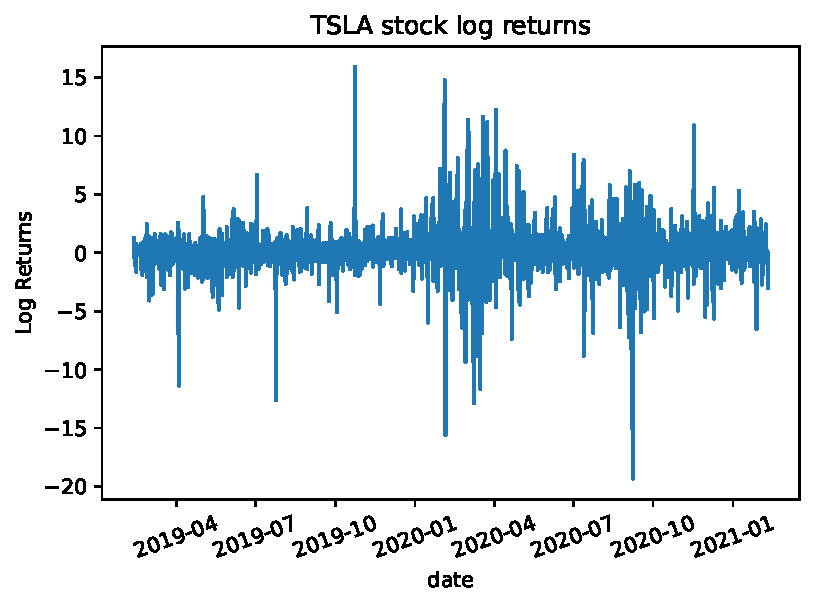
\includegraphics[width=\textwidth]{img/img_returns.pdf}
	\caption{Log returns of TSLA hourly opening stock price}
	\label{fig:tsla_returns}
\end{figure}

As financial data is not stationary and exhibits non-linear trends, and potentially heteroskedasticity, it is common practice to consider the log returns of the series. That is, to consider the series $X'_{t+1} = 100[ln(X_{t+1})-ln(X_t)]$. We see that in Fig \ref{fig:tsla_returns} the returns seem to be stationary. We check this by considering the \acrshort{acf} and \acrshort{pacf} graphs of the returns.

\begin{figure}
	\centering
	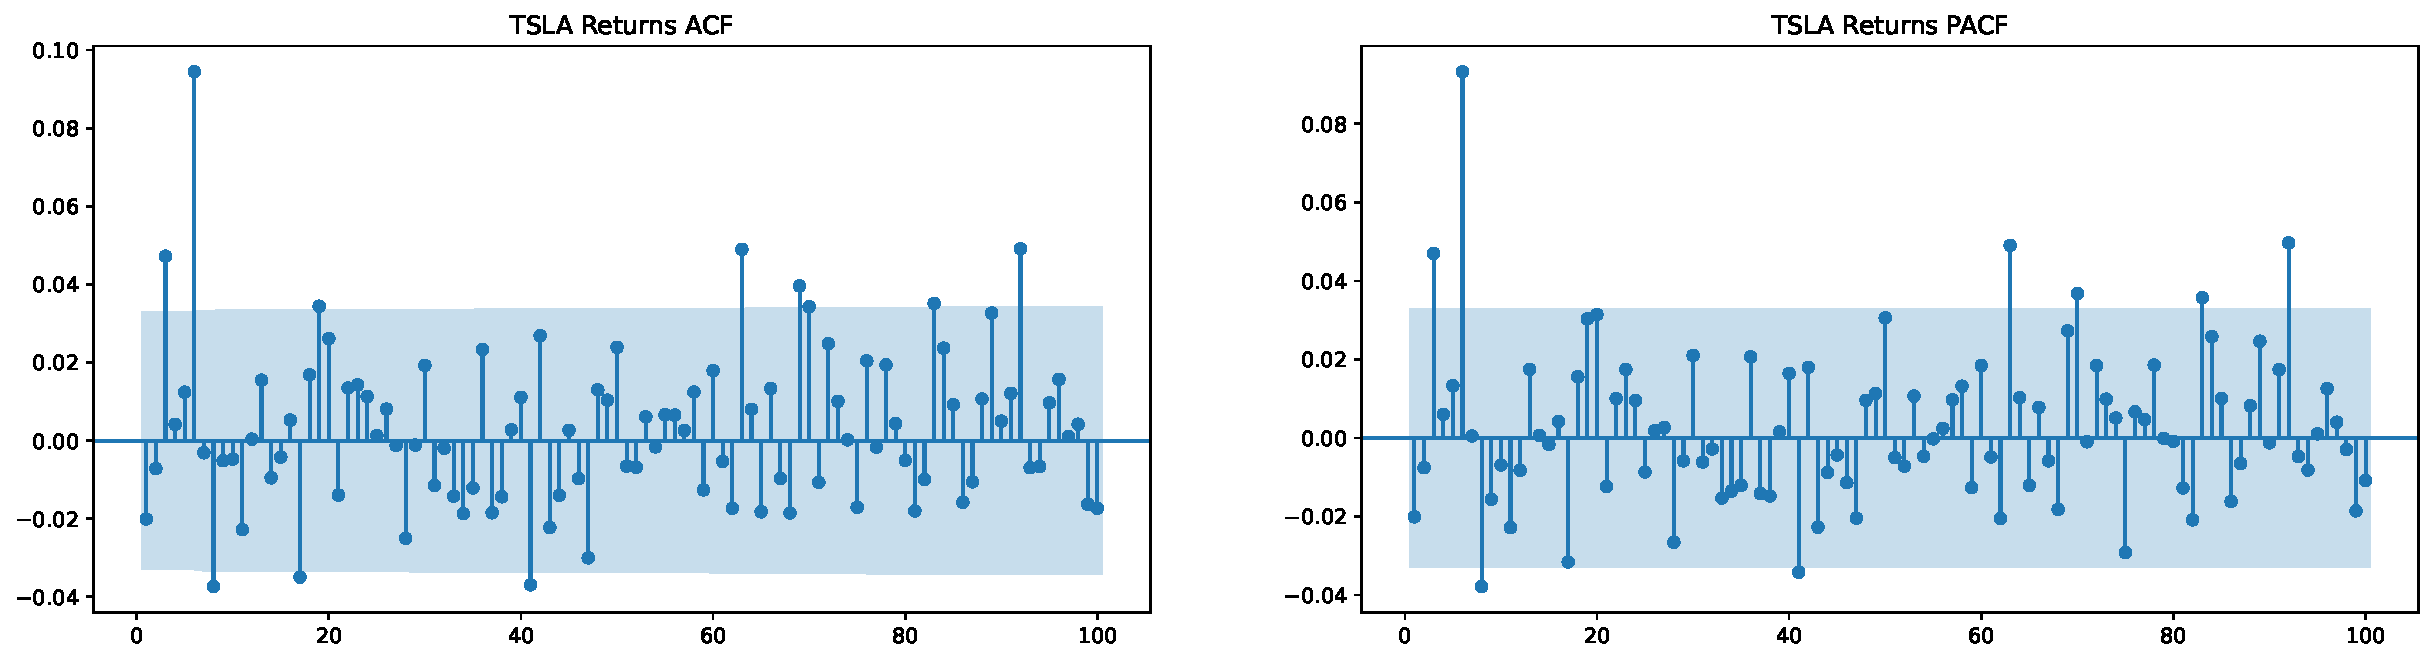
\includegraphics[width=\textwidth]{img/img_acf_tsla.pdf}
	\caption{\acrshort{acf} plot of log returns of TSLA stock price}
	\label{fig:acf_returns}
\end{figure}

Looking at Fig \ref{fig:acf_returns} there are a few lags that fall out of the 95\% significance interval. Oddly enough there would seem to be some significant autocorrelation at lag 6, which is surprising as if anything I would have expected there to be lag 7 autocorrelation, as there are 7 observations per day. It's not a very high autocorrelation nonetheless and fitting an \acrshort{arma} model with seasonality 6 just introduced more structure into the series instead of removing it, so we abandoned that path.

\begin{figure}
	\centering
	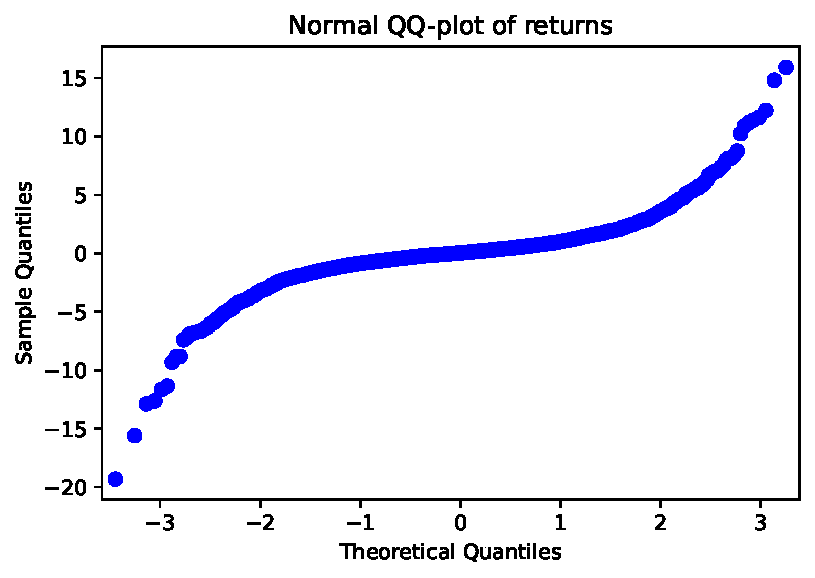
\includegraphics[width=\textwidth]{img/img_nqq_returns.pdf}
	\caption{Normal QQ plot of log returns of TSLA stock price}
	\label{fig:nqq_returns}
\end{figure}

We also checked the normal QQ-plot of the returns (Fig \ref{fig:nqq_returns}) and they are clearly not normally distributed. They have heavier tails, so we fitted a Student t distribution, manually tuned to a parameter $\nu = 2.6$ (Fig \ref{fig:tqq_returns}). This fits pretty well. At this point one could almost argue that the returns are just white noise with Student $t_{\nu}$ distribution.

\begin{figure}
	\centering
	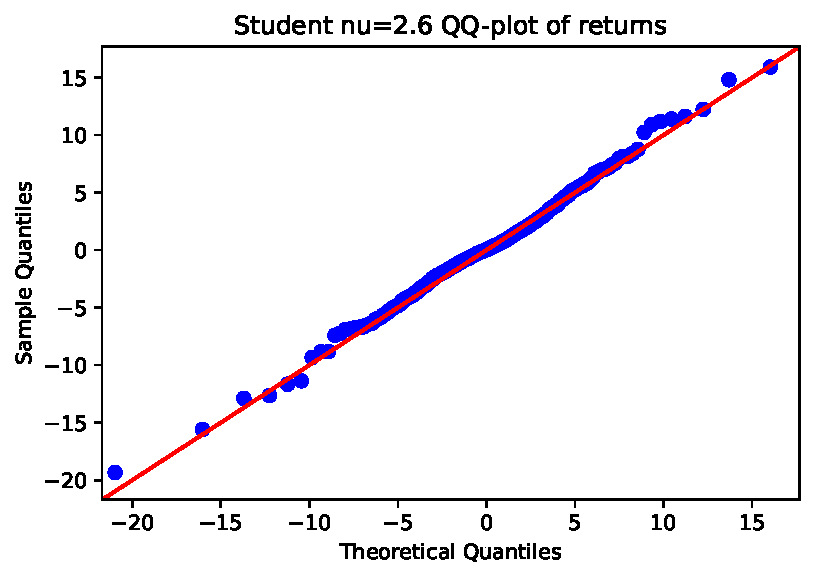
\includegraphics[width=\textwidth]{img/img_tqq_returns.pdf}
	\caption{Student QQ plot of log returns of TSLA stock price, with a parameter $\nu=2.6$}
	\label{fig:tqq_returns}
\end{figure}

However, when we look at the \acrshort{acf} and \acrshort{pacf} of the squared returns (Fig \ref{fig:acf_sreturns}, we notice distinct autocorrelation every lag multiple of 7. This suggest that there is significant structure in the volatility of the returns. This phenomena is called "volatility clustering" and happens a lot in financial \acrlong{ts}. The idea is that volatility breeds volatility; a period of volatility follows a period of volatility. 

\begin{figure}
	\centering
	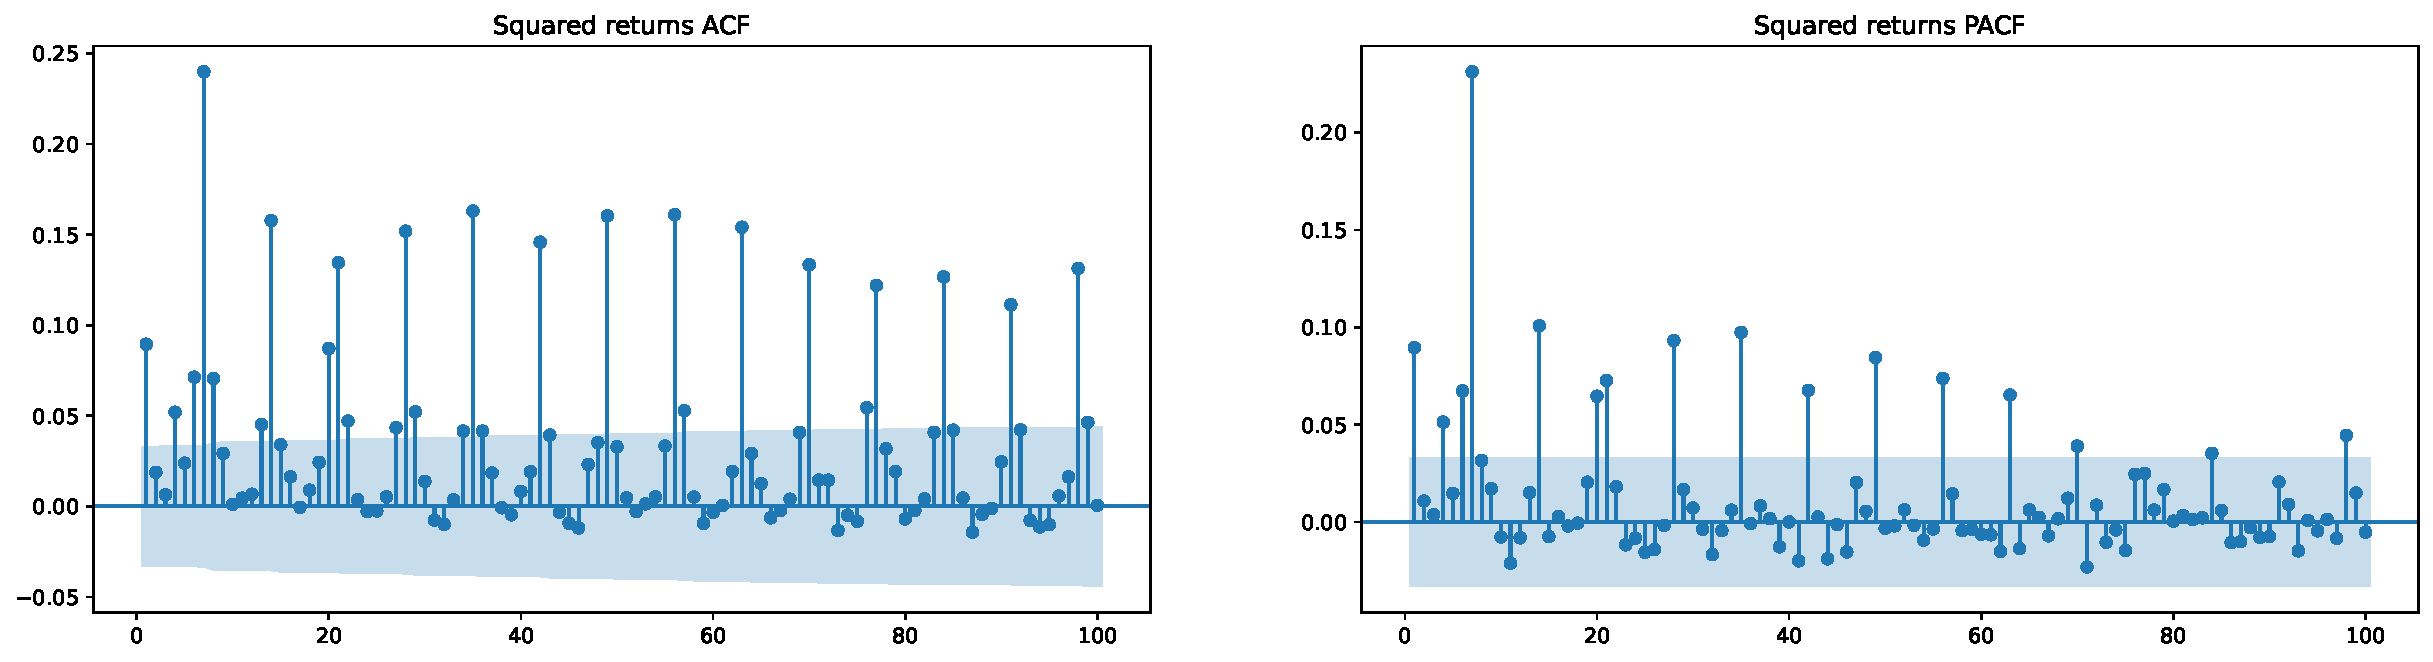
\includegraphics[width=\textwidth]{img/img_sreturns.pdf}
	\caption{\acrshort{acf} and \acrshort{pacf} of squared \acrshort{tsla} log returns}
	\label{fig:acf_sreturns}
\end{figure}

To model structure in the volatility of a series is where \acrshort{garch} model come into play. We first tried fitting a simple \acrshort{arch} model to the returns, but the results were not particularly better, so then we fit a \acrshort{garch}(1,1) with Student white noise model to the returns, and as you can see in figure \ref{fig:acf_sgarch} and figure \ref{fig:tqq_garch} the fit is very good.

\begin{figure}
	\centering
	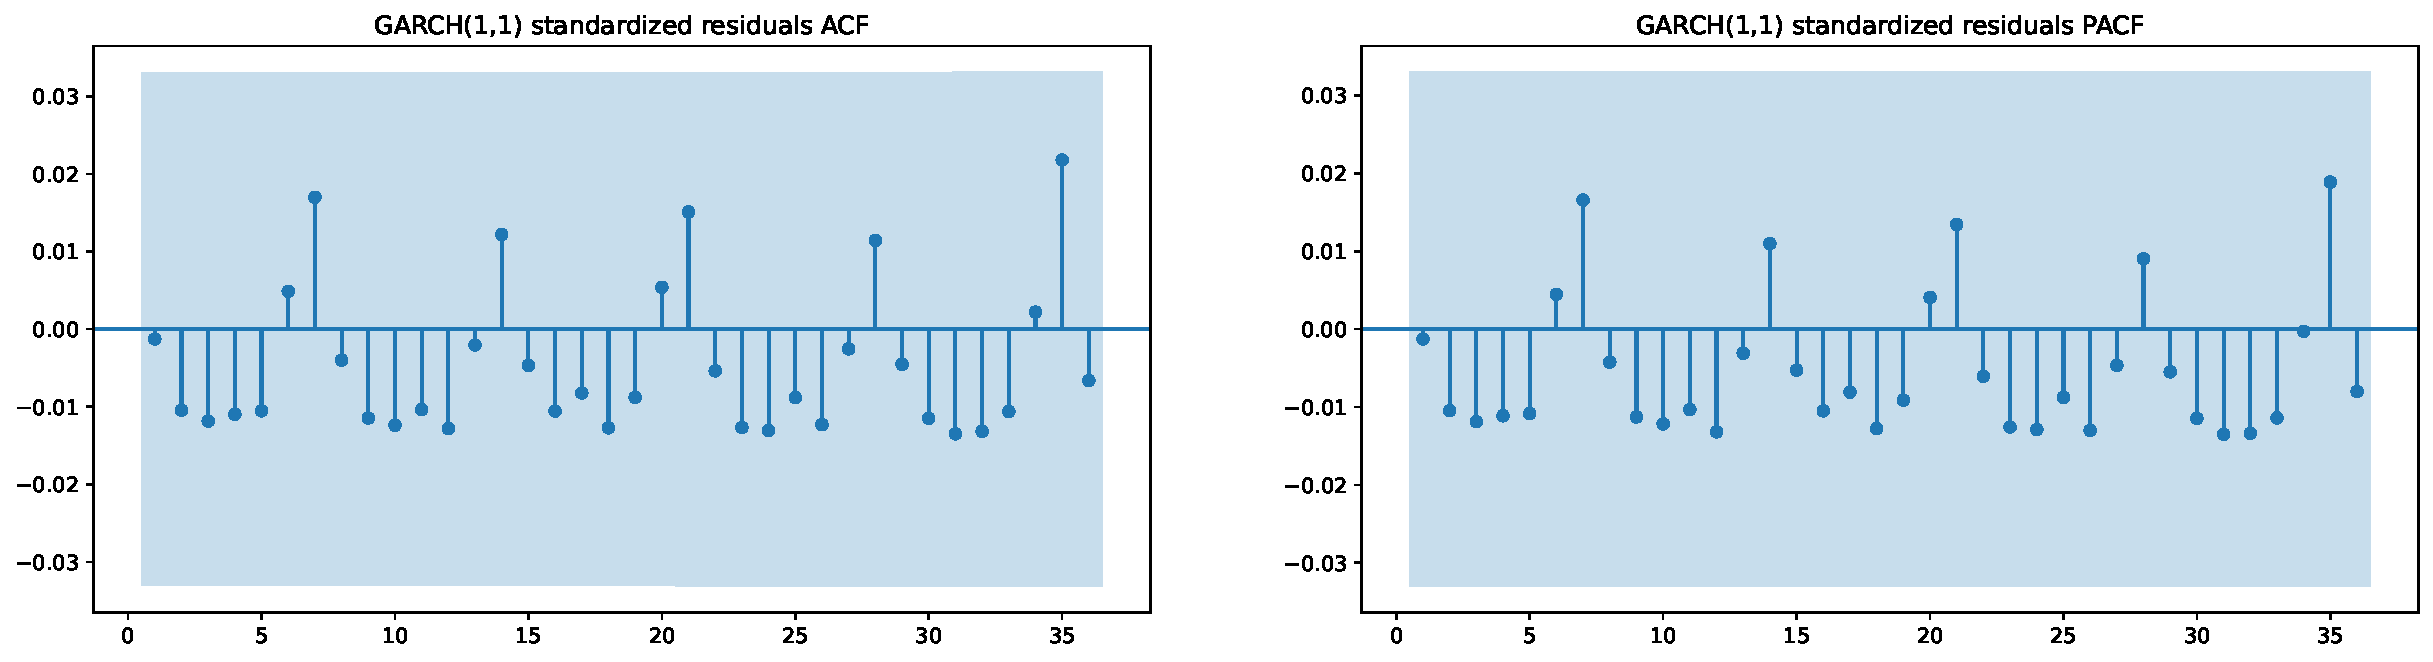
\includegraphics[width=\textwidth]{img/img_acf_garch.pdf}
	\caption{\acrshort{acf} and \acrshort{pacf} of squared standardized residuals from fitting a \acrshort{garch}(1,1) model with distribution $t_{\nu}$}
	\label{fig:acf_sgarch}
\end{figure}

\begin{figure}
	\centering
	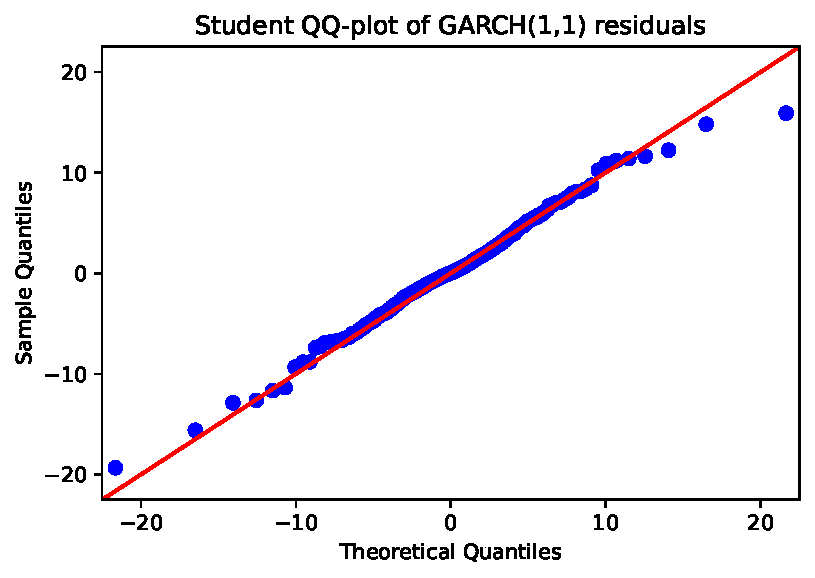
\includegraphics[width=\textwidth]{img/img_sqq_garch.pdf}
	\caption{Student QQ-plot of \acrshort{garch}(1,1) fitted to the \acrshort{tsla} returns}
	\label{fig:tqq_garch}
\end{figure}

The standardized residuals in figure \ref{fig:resid_garch} look very much like white noise now. Figure \ref{fig:resid_garch} also shows the conditional volatility extrapolated by the model. There are several things we see here. First, there is a large increase in volatility between January 2020 and May 2020, which I hypothesize is related to the uncertainty generated by the first wave of Covid-19. The later waves did not affect the volatility much, because by that time the initial panic had subsided, knowledge about the virus and how to fight it was more redly available. But that first wave caused havoc on the markets. The second thing we notice, is that there are spikes of very short duration but high value that happen every so often. They seem to be every 3-ish months and I would hypothesize that they more or less coincide with Tesla's quarterly earnings reports.
Indeed, according to Tesla's investors website ... \url{https://ir.tesla.com/}
The dates of the quarterly reports were:

\begin{tabular}{l}
Q4/18: Jan 30th 2019 \\
Q1/19: Apr 24th 2019 \\
Q2/19: Jul 24th 2019 \\% the website actually says Jun, which is a mistake. If clicked on it says Jul
Q3/19: Oct 23rd 2019 \\
Q4/19: Jan 29th 2020 \\
Q1/20: Apr 29th 2020 \\
Q2/20: Jul 22nd 2020 \\
Q3/20: Oct 21st 2020 \\
Q4/20: Jan 27th 2021
\end{tabular}


But this is not quite on point. First there is the case of Q1/20 which doesn't appear to have caused a spike in volatility, but this could just be that is was overshadowed by the Covid-19 first wave. Then there is Q4/20 that doesn't show up at the end of the graph. But as the other spikes are also a bit off from the quarterly report date, it's possible that the spike happens right after the end of the period we are considering, and that the spike are not fully explained by the quarterly report. Perhaps, when the spikes occur before the reports, it is because people are betting they will be good or bad, and there is excitement, maybe because a product launched that quarter or something. And when the spikes occur after the report, it could be because the reports were better or worse than expected, or maybe following a good report, Tesla or Elon Musk announce something big in the following days.
What's more, Tesla releases a press release basically 2 weeks prior to the earnings report. For Q4/18, this corresponds with the spike date.

As for the spike between Q2/20 and Q3/20, this could perhaps be explained by the stock split, which occurred on August 31st and fits relatively well. The first spike in November can be explained by the announcement that Tesla would be added to the \Gls{snp} index. Figure \ref{fig:volatility_garch} shows this.
\begin{figure}
	\centering
	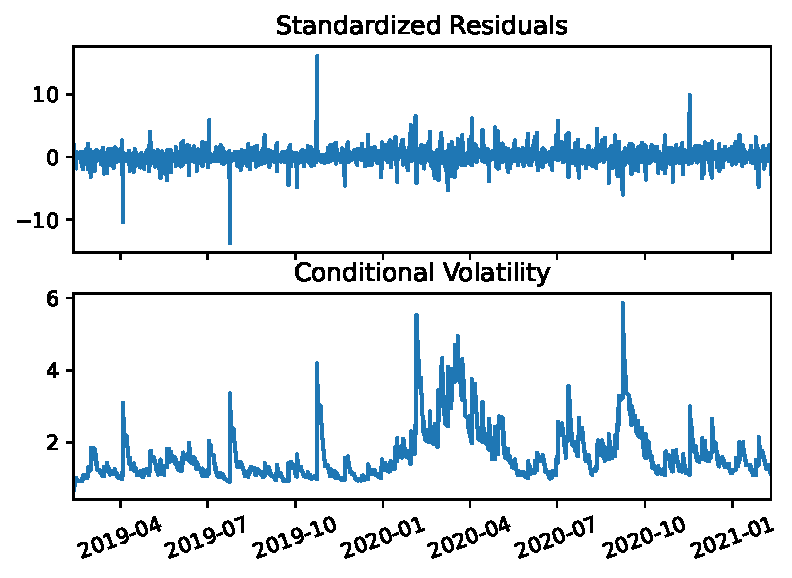
\includegraphics[width=\textwidth]{img/img_resid_garch.pdf}
	\caption{Standardized residual of the \acrshort{garch} fitting process and conditional volatility}
	\label{fig:resid_garch}
\end{figure}

\begin{figure}
	\centering
	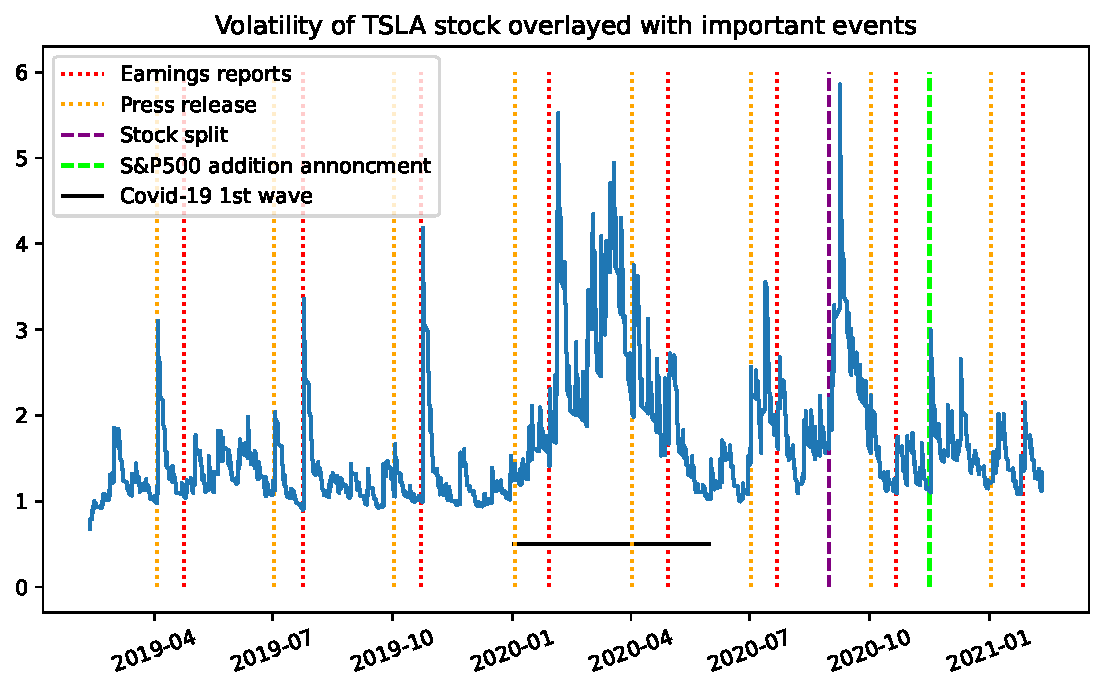
\includegraphics[width=\textwidth]{img/img_volatility_explanation.pdf}
	\caption{Important events overlayed with the \acrshort{garch} volatility}
	\label{fig:volatility_garch}
\end{figure}


The final \acrshort{ts} model is a \acrshort{garch}(1,1) model with Student-t distributed residuals. The parameters estimated by Python are:
\begin{align*}
\alpha_0 &= 0.042 \\
\alpha_1 &= 0.065 \\
\beta_1 &= 0.934 \\
\nu &= 2.56
\end{align*}
The parameters estimated by R are:
\begin{align*}
\alpha_0 &= 0.067 \\
\alpha_1 &= 0.137 \\
\beta_1 &= 0.935 \\
\nu &= 2.23 \\
\end{align*}

So there are some slight differences between the R and Python implementations, but the results are close. This could be explained by a difference of initial values for the solver


\section{Machine Learning Approach}